\documentclass{beamer}
\usepackage{listings}
\usetheme{Madrid}
\usecolortheme{seahorse}
\lstset{
%language=C,
frame=single, 
breaklines=true,
columns=fullflexible
}
\usepackage{subcaption}
\usepackage{url}
\usepackage{tikz}
\usepackage{amsmath}
\usepackage{graphicx}
\usepackage{tkz-euclide} % loads  TikZ and tkz-base
%\usetkzobj{all}
\usetikzlibrary{calc,math}
\usepackage{float}
\newcommand\norm[1]{\left\lVert#1\right\rVert}
\renewcommand{\vec}[1]{\mathbf{#1}}
\newcommand{\comb}[2]{{}^{#1}\mathrm{C}_{#2}}

\newcommand{\R}{\mathbb{R}}
\newcommand{\C}{\mathbb{C}}
\newcommand{\Beta}{B}
\newcommand{\Int}{\int\limits}
\providecommand{\brak}[1]{\ensuremath{\left(#1\right)}}
\providecommand{\abs}[1]{\vert#1\vert}
\providecommand{\fourier}{\overset{\mathcal{F}}{ \rightleftharpoons}}
\providecommand{\pr}[1]{\ensuremath{\Pr\left(#1\right)}}
\providecommand{\sbrak}[1]{\ensuremath{{}\left[#1\right]}}
\usepackage[export]{adjustbox}
\usepackage[utf8]{inputenc}
\usepackage{amsmath}
%environment for large proof
\makeatletter
\newenvironment<>{proofs}[1][\proofname]{%
    \par
    \def\insertproofname{#1\@addpunct{.}}%
    \usebeamertemplate{proof begin}#2}
  {\usebeamertemplate{proof end}}
\makeatother

\title{Research Paper Presentation}
\author{MANIKANTA VALLEPU}
\date{AI20BTECH11014}
\begin{document}
%
\begin{frame}
\titlepage
\end{frame}
%slide 2
\begin{frame}
\begin{block}{Topic}
A Probability-Based Analytical Model Based on Deep Learning for Traffic Information Estimation
\end{block}
\begin{block}{Authors}
\begin{enumerate}[]
\item Zhaoshan Sun,Fujian University of Technology, Fuzhou City, Fujian Province, China
\item Jeng-Shyang Pan , Fujian University of Technology, Fuzhou City, Fujian Province,Shandong University of Science and Technology, Qingdao City, Shandong Province, China
\item Chi-Hua Chen, Fuzhou University, Fuzhou City, Fujian Province, China
\item Tsu-Yang Wu, Shandong University of Science and Technology, Qingdao City, Shandong Province, China
\end{enumerate}
\end{block}
\begin{block}{Year of Publication}
   2020.
\end{block}
\end{frame}
%slide 3
\begin{frame}
\begin{block}{Abstract}
\begin{enumerate}[]
\item We will determine the PDF model based on deep learning to analyze the relationships between the number of call arrivals and vehicle speed.
\item We will discuss about vehicle speed estimation method to estimate vehicle speed in accordance with the number of call arrivals.
\item  We will study traffic flow estimation method to estimate traffic flow in accordance with the number of normal location updates.
\item We will also study traffic density estimation method to estimate the traffic density in accordance with the estimated vehicle speed and the estimated traffic flow.
\item Finally we will check accuracy of the model using simulation results.
\end{enumerate}
 \end{block}
\end{frame}
%slide 4
\begin{frame}{}
\begin{block}{Error function}
\begin{enumerate}[]
\item Also called the Gauss error function and denoted by erf. 
\item A Complex function of a complex variable defined as:
\begin{align}
       erf(x) =
       \frac{2}{\sqrt{\pi}}\int_{0}^{x}{e^{-t^{2}}}\,dt
\end{align}
\item This integral is a special (non-elementary) sigmoid function
\begin{figure}
    \centering
    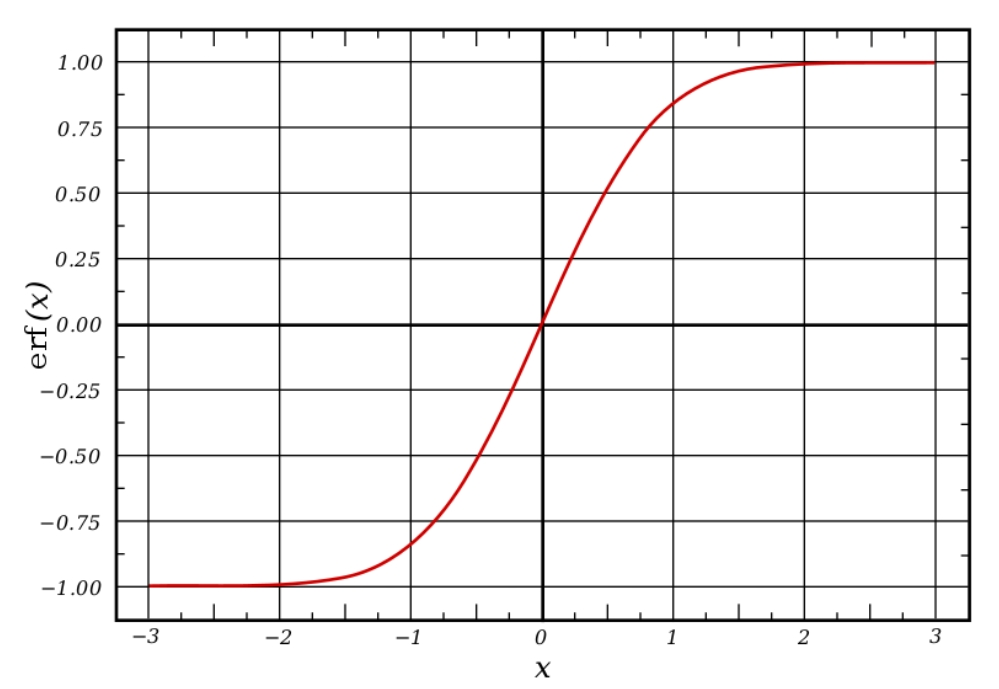
\includegraphics[scale=0.15]{erf.jpeg}
    \caption{Plot of the Error function} 
\end{figure}
\end{enumerate}
\end{block}
\end{frame}
%slide 5
\begin{frame}{}
\begin{block}{Error function contd}
\begin{enumerate}[]
\item Occurs oftenly in probability, statistics, and partial differential equations.
\item Estimate results that hold with high probability or low probability.
\item Given a random variable  $X\sim Norm[\mu , \sigma]$  and constant $L < \mu$:
\begin{align}
\pr{X\leq L} = \frac{1}{2} + \frac{1}{2} erf\brak{\frac{L - \mu}{\sqrt{2}\sigma}}
\end{align}
\end{enumerate}
\end{block}
\begin{block}{PTV VISSIM}
\begin{enumerate}[]
\item A microscopic multi-modal traffic flow simulation software package.
\item Complete software package for traffic analyses, forecasts and GIS-based data management on city, regional or national levels.
\end{enumerate}
\end{block}
\end{frame}
%slide 6
\begin{frame}{TRAFFIC INFORMATION ESTIMATION}
\begin{block}{Introduction}
\begin{enumerate}[]
\item Due to advance in science and technology, the intelligent transportation system (ITS) is becoming more powerful.
\item Real-time traffic information plays a significant role in ITS.
\item  The methods to gather real-time traffic information are divided into three categories:
\begin{enumerate}
\item Vehicle detectors (VDs)
\item Global position system (GPS)
\item Cellular floating vehicle data (CFVD).
\end{enumerate}
\item Compared with other two methods, CFVD is characterized by low cost and large data volume and can also avoid privacy issues.
\end{enumerate}
\end{block}
\end{frame}
%slide 7
\begin{frame}{TRAFFIC INFORMATION ESTIMATION}
\begin{block}{Cellular floating vehicle data (CFVD)}
\begin{enumerate}[]
\item CFVD is a method to determine the traffic speed on the road network based on the collection of localization data from mobile phones in vehicles that are being driven.
\item It collects the traffic information by  tracking the movements of mobile stations (MSs) using cellular network signals.
\item Some of the mainly used cellular network signals:
\begin{enumerate}
\item Normal Location Update (NLU)
\item Handover(HO)
\item Call Arrival (CA)
\end{enumerate}
\end{enumerate}
\end{block}
\end{frame}
%slide 8
\begin{frame}{ Vehicle Speed Estimation}
\begin{block}{Probability-Based Analysis}
\begin{enumerate}[]
\item Adopts the number of CAs to estimate vehicle speed.
\item Relationships between the number of CAs and traffic information were modelled in accordance with probability functions.
\item The distribution of call inter-arrival time was assumed to be an exponential distribution.However, the practical distribution may be not an exponential distribution.
\item Therefore, it uses deep learning techniques and adopts CDFs of exponential distribution, normal distribution and log-normal distribution to learn the CDF of call inter-arrival time.
\item The call inter-arrival time is adopted as the input of neural network, and the CDF is adopted as the output of neural network.
\end{enumerate}
\end{block}
\end{frame}
%slide 9
\begin{frame}{ Vehicle Speed Estimation}
\begin{block}{Probability-Based Analysis contd}
\begin{enumerate}[]
\item As shown in Figure, a  mobile station(MS) in the car moving along the road performs the first call set-up (at time $t_0$) and then enters $Cell_i$ coverage (at time $t_1$). It subsequently performs the second call set-up (at time $t_2$) before leaving $Cell_i$ coverage (at
time $t_3$).
\begin{figure}
    \centering
    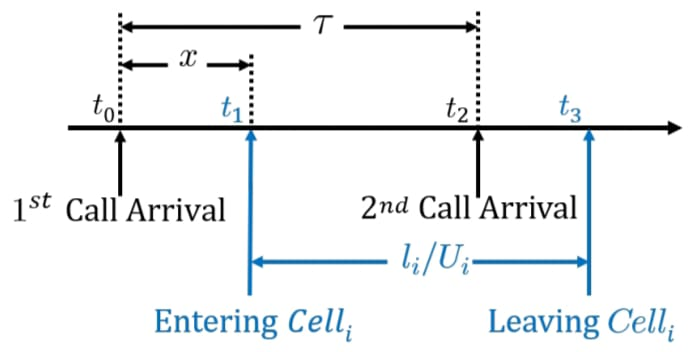
\includegraphics[scale=0.25]{fig_p.jpeg}
    \caption{The timing diagram for vehicle movement and CA on the road} 
\end{figure}
\end{enumerate}
\end{block}
\end{frame}
%slide 10
\begin{frame}{Vehicle Speed Estimation}
\begin{block}{Probability-Based Analysis contd}
\begin{enumerate}[]
\item Using deep learning techniques and adopting the  CDFs of exponential distribution, normal distribution and log-normal distribution, the relationship between the number of CAs and vehicle speed is expressed as Equation \eqref{3}.
\item Some of the notations used in the equation are :
    \begin{enumerate}[]
     \item The practical vehicle speed, traffic flow and traffic density of $Cell_i$ are denoted as $U_i$, $Q_i$ and $K_i$.
     \item  The number of CAs of $Cell_i$ is denoted $r_i$.
     \item The parameters ${\mu}_1$, ${\mu}_2$, ${\mu}_3$, ${\sigma}_2$ and ${\sigma}_3$ are the weights of the proposed activation functions in the neural network.
     \end{enumerate}
\end{enumerate}
\end{block}
\end{frame}
%slide 11
\begin{frame}{ Vehicle Speed Estimation}
\begin{block}{Probability-Based Analysis contd}
\begin{multline}
r_i = Q_i \times \pr{t_1 < t_2 < t_3}\\
= \mu_1\brak{1 - e^{- \frac{1}{\mu_1}\brak{\frac{1}{u_i}}}} + \frac{l}{2 u_i} - \frac{1}{2}\brak{\frac{l}{u_i} - \mu_2}erf\brak{\frac{\frac{l}{u_i} - \mu_2}{\sigma_2 \sqrt{2}}} + \\\brak{-\frac{1}{2 \mu_2}}erf\brak{\frac{- \mu_2}{\sigma_2 \sqrt{2}}}
-\frac{\sigma_2 \sqrt{2} e^{-\brak{\frac{l^{2} - l_2}{\frac{\sigma_2}{2}}}^{2}}}{2 \sqrt{\pi}} \frac{\sigma_2 \sqrt{2} e^{-\brak{\frac{\mu_2}{\frac{\sigma_2}{2}}}^{2}}}{2 \sqrt{\pi}}\\+ \frac{l}{2 u_i} - \frac{1}{2} e^{\mu_3 + \frac{\sigma_2^{2}}{2}}\brak{erf\brak{\frac{-\ln{\frac{l}{u_i}} + \mu_3 + \sigma_3^{2}}{\sigma_3 \sqrt{2}}} - 1}\\
- \brak{\frac{l}{2 u_i}}erf\brak{\frac{\ln{\frac{l}{u_i}} - \mu_3}{\sigma_3 \sqrt{2}}} \label{3}
\end{multline}
\end{block}
\end{frame}
%slide 12
\begin{frame}{ Vehicle Speed Estimation}
\begin{block}{ Estimation Based on Deep Learning}
\begin{enumerate}[]
\item The probability-based analytical model indicates
that the relationship between the number of CAs and vehicle
speed is significant.
\item Trains another neural network to estimate vehicle speed in accordance with the number of CAs.
\item The input is the number of CAs and vehicle
speed is adopted as the output of neural network.
\end{enumerate}
\end{block}
\end{frame}
%slide 13
\begin{frame}{}
\begin{block}{Traffic Flow Estimation}
\begin{enumerate}[]
\item Assumes that the actual traffic flow on the road segment covered by $Cell_i$
is $Q_i$ and one MS is in each vehicle.
\item The NLU event is generated when an MS moves from a location area (LA)
to another LA.
\item The number of NLUs ($q_i$) is equal to traffic flow ($Q_i$) while a vehicle is passing through a LA.
 \begin{align}
 q_i = Q_i \label{4}
 \end{align}
\end{enumerate}
\end{block}
\begin{block}{ Traffic Density Estimation}
\begin{enumerate}[]
\item Denoted by $k_i$ and estimated according to the estimated vehicle speed ($u_i$) and the estimated traffic flow ($q_i$).
\item  The traffic density ($k_i$) is given by the equation \eqref{2}, 
\begin{align}
k_i = \frac{q_i}{u_i} \label{2}
\end{align}
\end{enumerate}
\end{block}
\end{frame}
%slide 14
\begin{frame}{}
\begin{block}{SIMULATION ANALYSIS}
\begin{enumerate}[]
\item The practical traffic information were adopted as simulation data in this study.
\item The practical information contained road conditions and
vehicle movement behaviors.
\item The vehicle movements were generated by VISSIM.
\item Assumptions according to the statistical results:
        \begin{enumerate}[]
        \item $l_i$=1.0 km
        \item $\mu_i$ =1 call/h
        \end{enumerate}
\item Generates random numbers of call inter-arrival time with normal distribution for each MS.
\item The accuracies of vehicle speed estimation and traffic density
estimation are described as $1 -\frac{\abs{U_i - u_i}}{U_i}$
and $1 -\frac{\abs{K_i - k_i}}{K_i}$.
\end{enumerate}
\end{block}
\end{frame}
%slide 15
\begin{frame}{}
\begin{block}{SIMULATION ANALYSIS contd}
   \begin{center}
\begin{table}[h]
    \centering
    \scalebox{0.65}{
    \resizebox{\columnwidth}{!}{
\begin{tabular}{|c|c|c|c|c|c|c|}
\hline
\textbf{Cell} & \textbf{$U_i$} & \textbf{$K_i$} & \textbf{$u_i$} & \textbf{$k_i$} & \textbf{$1 -\frac{\abs{U_i - u_i}}{U_i}$} & \textbf{$1 -\frac{\abs{K_i - k_i}}{K_i}$} \\
\hline
1 & 81.27 & 64 & 80.06 & 64.65 & 96.13\% & 95.98\% \\ 
\hline
2 & 80.68 & 64.37 & 80.83 & 63.98 & 96.71\% & 96.95\% \\
\hline
3 & 80.29 & 64.68 & 79.86 & 64.79 & 96.66\% & 96.73\% \\
\hline
4 & 80.06 & 64.84 & 80.51 & 64.21 & 95.46\% & 95.59\% \\
\hline
5 & 79.92 & 64.98 & 79.76 & 64.84 & 96.73\% & 96.72\% \\
\hline
6 & 79.8 & 65.08 & 78.88 & 65.59 & 96.74\% & 96.93\% \\
\hline
7 & 79.69 & 65.19 & 79.99 & 64.66 & 96.42\% & 96.51\% \\
\hline
8 & 79.58 & 65.28 & 80.27 & 64.43 & 96.50\% & 96.66\% \\
\hline
9 & 79.57 & 65.31 & 80.32 & 64.29 & 95.35\% & 95.62\% \\
\hline
10 & 79.48 & 65.38 & 79.73 & 65.07 & 96.85\% & 96.80\% \\
\hline
average &  &  &  &  & 96.36\% & 96.45\% \\
\hline
\end{tabular}
}
}
    \caption{SIMULATION RESULT}
    \label{table 1}
\end{table}
\end{center}
From the above Table, the accuracies of estimated vehicle speed and
estimated traffic density were 96.36\% and 96.45\%.
\end{block}
\end{frame}
%slide 16
\begin{frame}
   \centering
    \textcolor{blue}{\Huge{\textbf{THANK YOU}}}
\end{frame}

\end{document}